\state{Twins paradox (MCP 2.16)}{\hfix}

\prob{
	The 4-acceleration of a particle or other object is defined by $\vaa \equiv \dv*{\vuu}{\tau}$, where $\vuu$ is its 4-velocity and $\tau$ is proper time along its world line.  Show that, if an observer carries an accelerometer, the magnitude $\abs{\ba}$ of the 3-dimensional acceleration $\ba$ measured by the accelerometer will always be equal to the magnitude of the observer's 4-acceleration, $\abs{\ba} = \abs{\vaa} \equiv \sqrt{\vaa \cdot \vaa}$.
}

\sol{
	The accelerometer will display the acceleration as measured in its instantaneous rest frame.  From MCP~(2.25c), its 4-velocity can be written
	\eq{
		\vuu = (\gam, \gam \bv)
		= \gam (1, \bv),
	}
	where $\bv = \dv*{\xbb}{t}$ and $\xbb$ is the position in 3-space.  Then the acceleration is
	\eq{
		\vaa = \dv{\vuu}{\tau}
		= \gam \dv{\vuu}{t}
		= \gam \paren{ \dv{\gam}{t}, \bv \dv{\gam}{t} + \gam \dv{\bv}{t} },
	}
	since $\ddtau = \ddt / \gam$~\cite[p.~201]{Resnick}.  But in the instantaneous rest frame of the accelerometer and observer, $\gam = 1$ and $\dv*{\gam}{t} = 0$.  So the accelerometer measures
	\eq{
		\vaa = \paren{ 0, \dv{\bv}{t} }
		= (0, \ba).
	}
	Then
	\eq{
		\ans{ \abs{\vaa} = \sqrt{ \vaa \cdot \vaa }
		= \sqrt{ \ba \vdot \ba }
		= \abs{\ba}, }
	}
	as we wanted to show. \qed
}


\prob{
	In the twins paradox of Fig.~2.8a, suppose that Florence begins at rest beside Methuselah, then accelerates in Methuselah's $x$-direction with an acceleration $a$ equal to one Earth gravity, $g$, for a time $\TFlo / 4$ as measured by her, then accelerates in the $-x$-direction at $g$ for a time $\TFlo / 2$, thereby reversing her motion; then she accelerates in the $+x$-direction at $g$ for a time $\TFlo / 4$, thereby returning to rest beside Methuselah.  (This is the type of motion shown in the figure.)  Show that the total time lapse as measured by Methuselah is
	\eq{
		\TMet = \frac{4}{g} \sinh(\frac{g \TFlo}{4}).
	}
}

\sol{
	Let $a$ be Florence's acceleration as measured in Methuselah's rest frame $\cF$.  For the first quarter of her journey, Florence's proper acceleration is $\ab = g$.  The expression for the Lorentz transformation relating the proper acceleration is~\cite{Acceleration}
	\eq{
		\ab = \frac{a}{(1 - \bet^2)^{3/2}}.
	}
	Rearranging and substituting yields (for $c = 1$)
	\eq{
		a = g (1 - \bet^2)^{3/2}
		= g (1 - v^2)^{3/2},
	}
	where $v$ is Florence's velocity as observed by Methuselah.  Substituting $a = \dv*{v}{t}$ gives us a differential equation for $v$:
	\eq{
		\dv{v}{t} = g (1 - v)^{3/2}
		\qimplies
		\intov \frac{\ddvp}{(1 - {v'}^2)^{3/2}} = g \intot \ddtp
		\qimplies
		\frac{v}{\sqrt{1 - v^2}} = g t,
	}
	where Florence begins her journey at time 0 in both inertial frames, and Florence's initial velocity is 0 in both.  (This integral and all following computations in this problem are performed using Mathematica.)  Solving for $v$ yields
	\eqn{v1}{
		v = \frac{g t}{\sqrt{1 + (g t)^2}}.
	}
	Now we relate time in both frames using $\ddtau = \ddt / \gam$~\cite[p.~201]{Resnick}.  Here, $\tau$ is the time Florence measures in her rest frame, and $t$ is the time in Methuselah's rest frame.  Both measure the initial time as 0.  Then
	\eq{
		\int \ddtau = \int \frac{\ddt}{\gam}
		\qimplies
		\tau = \int \sqrt{1 - v^2} \ddt
		= \int \sqrt{1 - \frac{(g t)^2}{1 + (g t)^2}} \ddt
		= \frac{1}{g} \int \sqrt{1 - \frac{u^2}{1 + u^2}} \ddu.
	}
	Let $\TMetq$ be the time in Methuselah's rest frame at the end of the first quarter of Florence's trip.  We find
	\eq{
		\frac{\TFlo}{4} = \frac{1}{g} \int_0^{g \TMetq} \sqrt{1 - \frac{u^2}{1 + u^2}} \ddt
		= \frac{\sinh[-1](g \TMetq)}{g},
	}
	which implies~\cite{Muller}
	\eqn{Met4}{
		\TMetq = \frac{1}{g} \sinh(\frac{g \TFlo}{4}).
	}
	Now we consider the second quarter of Florence's journey.  At $\tau = \TFlo / 4$, her acceleration switches direction but does not change in magnitude.  This means her motion over the next time interval of $\TFlo / 4$ looks like the first quarter of her trip played in reverse.  This is also what Methuselah sees.  So at the instant $\tau = \TFlo / 2$ and $t = 2 \TMetq$, she will be back at her starting point with velocity 0.
	
	At this instant we are at the halfway point of Florence's journey.  The second half of her journey plays out exactly like the first, except it is the mirror image.  Thus, it must take exactly the same amount of time as the first half.  So the total length of the journey is $\TFlo$ for Florence, and $4 \TMetq$ for Methuselah.  From Eq.~\refeq{Met4}, then, we have
	\eqn{show5b}{
		\ans{ \TMet = \frac{4}{g} \sinh(\frac{g \TFlo}{4}) }
	}
	as we wanted to show. \qed
}


\prob{
	Show that in the geometrized units used here, Florence's acceleration (equal to acceleration of gravity at the surface of Earth) is $g = \SI{1.033}{\per\year}$.  Plot $\TMet$ as a function of $\TFlo$, and from your plot estimate $\TFlo$ if $\TMet$ is the age of the Universe, 14 billion years.
}

\sol{
	Note that
	\eq{
		c = 1
		\approx \SI{2.998e8}{\meter\per\second}
		\qimplies
		\SI{1}{\meter} \approx \frac{1}{\num{2.998e8}} \, \si{\second}
		\approx \SI{3.336e-9}{\second}.
	}
	Using this relation to convert $g$ from SI units, as well as the fact that $\SI{1}{\year} \approx \SI{3.154e7}{\second}$,
	\eq{
		g = \SI{9.807}{\meter\per\square\second}
		= (\SI{9.807}{\per\square\second}) (\SI{3.336e-9}{\second})
		= (\SI{3.271e-8}{\per\second}) (\SI{3.154e7}{\second\per\year})
		\approx \ans{ \SI{1.033}{\per\year}, }
	}
	as we wanted to show. \qed
	
	Figure~\ref{f5} shows a plot of Eq.~\refeq{show5b}.  When $\TMet \approx \SI{14e9}{\year}$, $\TFlo \approx \ans{ \SI{88}{\year} }$.
	
	\begin{figure}[t] \centering
		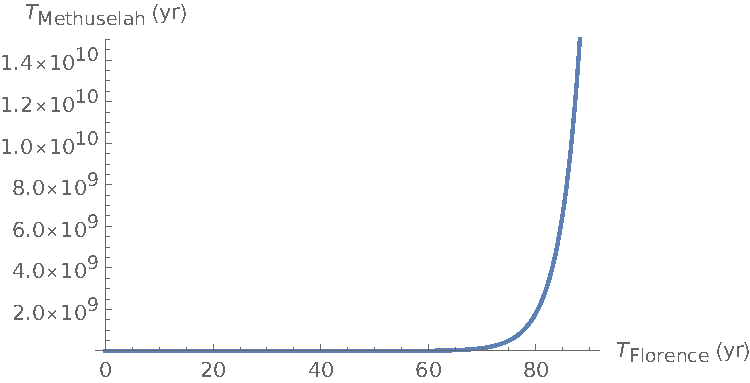
\includegraphics[width=0.5\textwidth]{5c}
		\caption{Plot of Eq.~\refeq{show5b} indicating $\TFlo$ when $\TMet \approx \SI{14e9}{\year}$.}
		\label{f5}
	\end{figure}
}